%%%%%%%%%%%%%%%%%%%%%%%%%%%%%%%%%%%%%%%%%
% Short Sectioned Assignment LaTeX Template Version 1.0 (5/5/12)
% This template has been downloaded from: http://www.LaTeXTemplates.com
% Original author:  Frits Wenneker (http://www.howtotex.com)
% License: CC BY-NC-SA 3.0 (http://creativecommons.org/licenses/by-nc-sa/3.0/)
%%%%%%%%%%%%%%%%%%%%%%%%%%%%%%%%%%%%%%%%%

%----------------------------------------------------------------------------------------
%	PACKAGES AND OTHER DOCUMENT CONFIGURATIONS
%----------------------------------------------------------------------------------------

\documentclass[paper=a4, fontsize=11pt]{scrartcl} % A4 paper and 11pt font size

% ---- Entrada y salida de texto -----

\usepackage[T1]{fontenc} % Use 8-bit encoding that has 256 glyphs
\usepackage[utf8]{inputenc}
%\usepackage{fourier} % Use the Adobe Utopia font for the document - comment this line to return to the LaTeX default

% ---- Idioma --------

\usepackage[spanish, es-tabla]{babel} % Selecciona el español para palabras introducidas automáticamente, p.ej. "septiembre" en la fecha y especifica que se use la palabra Tabla en vez de Cuadro

% ---- Otros paquetes ----

\usepackage{url} % ,href} %para incluir URLs e hipervínculos dentro del texto (aunque hay que instalar href)
\usepackage{hyperref}
\hypersetup{
	colorlinks=true,
	linkcolor=black,
	urlcolor=black,
	citecolor=black,
}
\usepackage{amsmath,amsfonts,amsthm} % Math packages
%\usepackage{graphics,graphicx, floatrow} %para incluir imágenes y notas en las imágenes
\usepackage{graphics,graphicx, float} %para incluir imágenes y colocarlas

% Para hacer tablas comlejas
%\usepackage{multirow}
%\usepackage{threeparttable}

%\usepackage{sectsty} % Allows customizing section commands
%\allsectionsfont{\centering \normalfont\scshape} % Make all sections centered, the default font and small caps

\usepackage{fancyhdr} % Custom headers and footers
\pagestyle{fancyplain} % Makes all pages in the document conform to the custom headers and footers
\fancyhead{} % No page header - if you want one, create it in the same way as the footers below
\fancyfoot[L]{} % Empty left footer
\fancyfoot[C]{} % Empty center footer
\fancyfoot[R]{\thepage} % Page numbering for right footer
\renewcommand{\headrulewidth}{0pt} % Remove header underlines
\renewcommand{\footrulewidth}{0pt} % Remove footer underlines
\setlength{\headheight}{13.6pt} % Customize the height of the header

\numberwithin{equation}{section} % Number equations within sections (i.e. 1.1, 1.2, 2.1, 2.2 instead of 1, 2, 3, 4)
\numberwithin{figure}{section} % Number figures within sections (i.e. 1.1, 1.2, 2.1, 2.2 instead of 1, 2, 3, 4)
\numberwithin{table}{section} % Number tables within sections (i.e. 1.1, 1.2, 2.1, 2.2 instead of 1, 2, 3, 4)

\setlength\parindent{0pt} % Removes all indentation from paragraphs - comment this line for an assignment with lots of text

\newcommand{\horrule}[1]{\rule{\linewidth}{#1}} % Create horizontal rule command with 1 argument of height

\usepackage{listings}
\usepackage{color}
\usepackage{xcolor}
\lstdefinestyle{customc}{
	belowcaptionskip=1\baselineskip,
	breaklines=true,
	frame=L,
	xleftmargin=\parindent,
	language=C,
	showstringspaces=false,
	basicstyle=\footnotesize\ttfamily,
	keywordstyle=\bfseries\color{green!40!black},
	commentstyle=\itshape\color{purple!40!black},
	identifierstyle=\color{blue},
	stringstyle=\color{orange},
}

\lstset{escapechar=@,style=customc}

\title{	
	\normalfont \normalsize 
	\textsc{\textbf{Inteligencia de Negocio} \\ Grado en Ingeniería Informática \\ Universidad de Granada \\
	Curso 2017-2018} \\ [25pt] % Your university, school and/or department name(s)
	\horrule{0.5pt} \\[0.4cm] % Thin top horizontal rule
	\huge Memoria Práctica 3. \\
	\huge Competición de Kaggle.
	\\ % The assignment title
	\horrule{2pt} \\[0.5cm] % Thick bottom horizontal rule
}

\author{Alberto Armijo  \\
\href{mailto:armijoalb@correo.ugr.es}{armijoalb@correo.ugr.es}} % Nombre y apellidos
\date{\normalsize\today} % Incluye la fecha actual

%----------------------------------------------------------------------------------------
% DOCUMENTO
%----------------------------------------------------------------------------------------

\begin{document}
	
	\maketitle % Muestra el Título
	
	\newpage %inserta un salto de página
	
	\tableofcontents % para generar el índice de contenidos
	
	\listoffigures % para generar índice de imágenes.
	
	\listoftables % para generar índice de tablas.
	
	\newpage
	
	\section[Introducción]{Introducción.}
	En esta práctica se explicarán los pasos seguidos durante la competición hasta conseguir el resultado que se puede ver en la clasificación.
	
	\vspace{0.06in}
	La competición de Kaggle se trata de resolver un problema de regresión para predecir el valor de una casa según un conjunto de características, como el número de habitaciones, el espacio que tiene el garaje, el espacio de cada una de las plantas de la vivienda, el año en que se construyo, etc...
	
	\vspace{0.06in}
	Para resolver el problema, se utilizarán algunos algoritmos que se han mostrado en la asignatura de prácticas, como por ejemplo XGBoost (Gradient Boosting).
	
	\section[Explicación]{Explicación código desarrollado.}
	En este apartado se explicarán las medidas tomadas a la hora de preprocesar los datos y ejecutar los diferentes algoritmos utilizados para predecir el valor de las viviendas.
	
	\vspace{0.06in}
	
	\subsection{Estudio de los datos.}
	Lo primero que tenemos que miré fue el tamaño de nuestro conjunto de datos, para el training contamos con 1460 datos y para el test contamos con 1459 datos.
	
	\vspace{0.06in}
	Lo siguiente que hice es comprobar comprobar las columnas que tienen valores perdidos y el porcentaje de valores perdidos por cada una de las variables. Estos son las variables con valores perdidos (en el conjunto de train).
	
	\begin{lstlisting}
	total = train.isnull().sum().sort_values(ascending=False)
	percent = (train.isnull().sum()/train.isnull().count()).sort_values(ascending=False)
	missing_data = pd.concat([total, percent], axis=1, keys=['Total', 'Percent'])
	missing_data = missing_data[missing_data['Total'] > 0]
	names = list(missing_data.index)
	sns.barplot(x=names,y='Percent',data=missing_data)
	plt.xticks(rotation=45)
	plt.savefig('missing_data.pdf')
	\end{lstlisting}
	
	\begin{figure}[H]
		\centering
		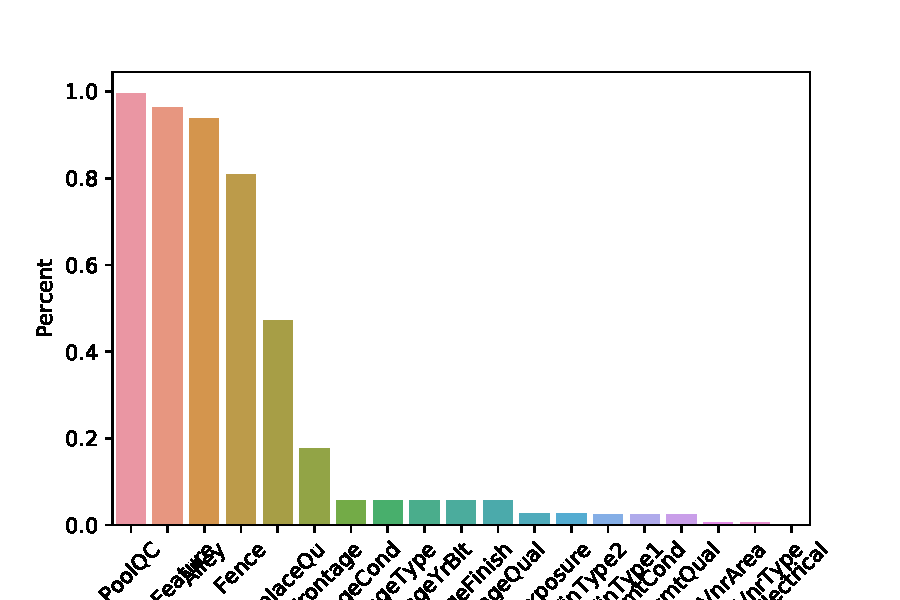
\includegraphics[scale=0.8]{imag/missing_data.pdf}
		\caption{Datos pérdidos en train}
		\label{fig:missing_data_train}
	\end{figure}
	
	\vspace{0.06in}
	
	Para todas estas variables tendremos o que borrar la variable o imputar los datos, eso se verá en el apartado de preprocesado de datos.
	
	\vspace{0.06in}
	
	Lo siguiente que haremos es ver que variables numéricas son las más importantes, y que variables categóricas son las más importantes conforme a la variable SalePrice.
	
	\vspace{0.06in}
	Para calcular las variables que están más correlacionadas, haremos una matriz de correlación, esto lo podemos hacer con pandas directamente. Después, crearemos un heatmap para representar las correlaciones entre las variables.
	
	\begin{lstlisting}
	f, ax = plt.subplots(figsize=(12, 9))
	corrmat = train.corr()
	sns.heatmap(corrmat)
	plt.xticks(rotation=45)
	plt.savefig('correlation.pdf')
	\end{lstlisting}
	
	\begin{figure}[H]
		\centering
		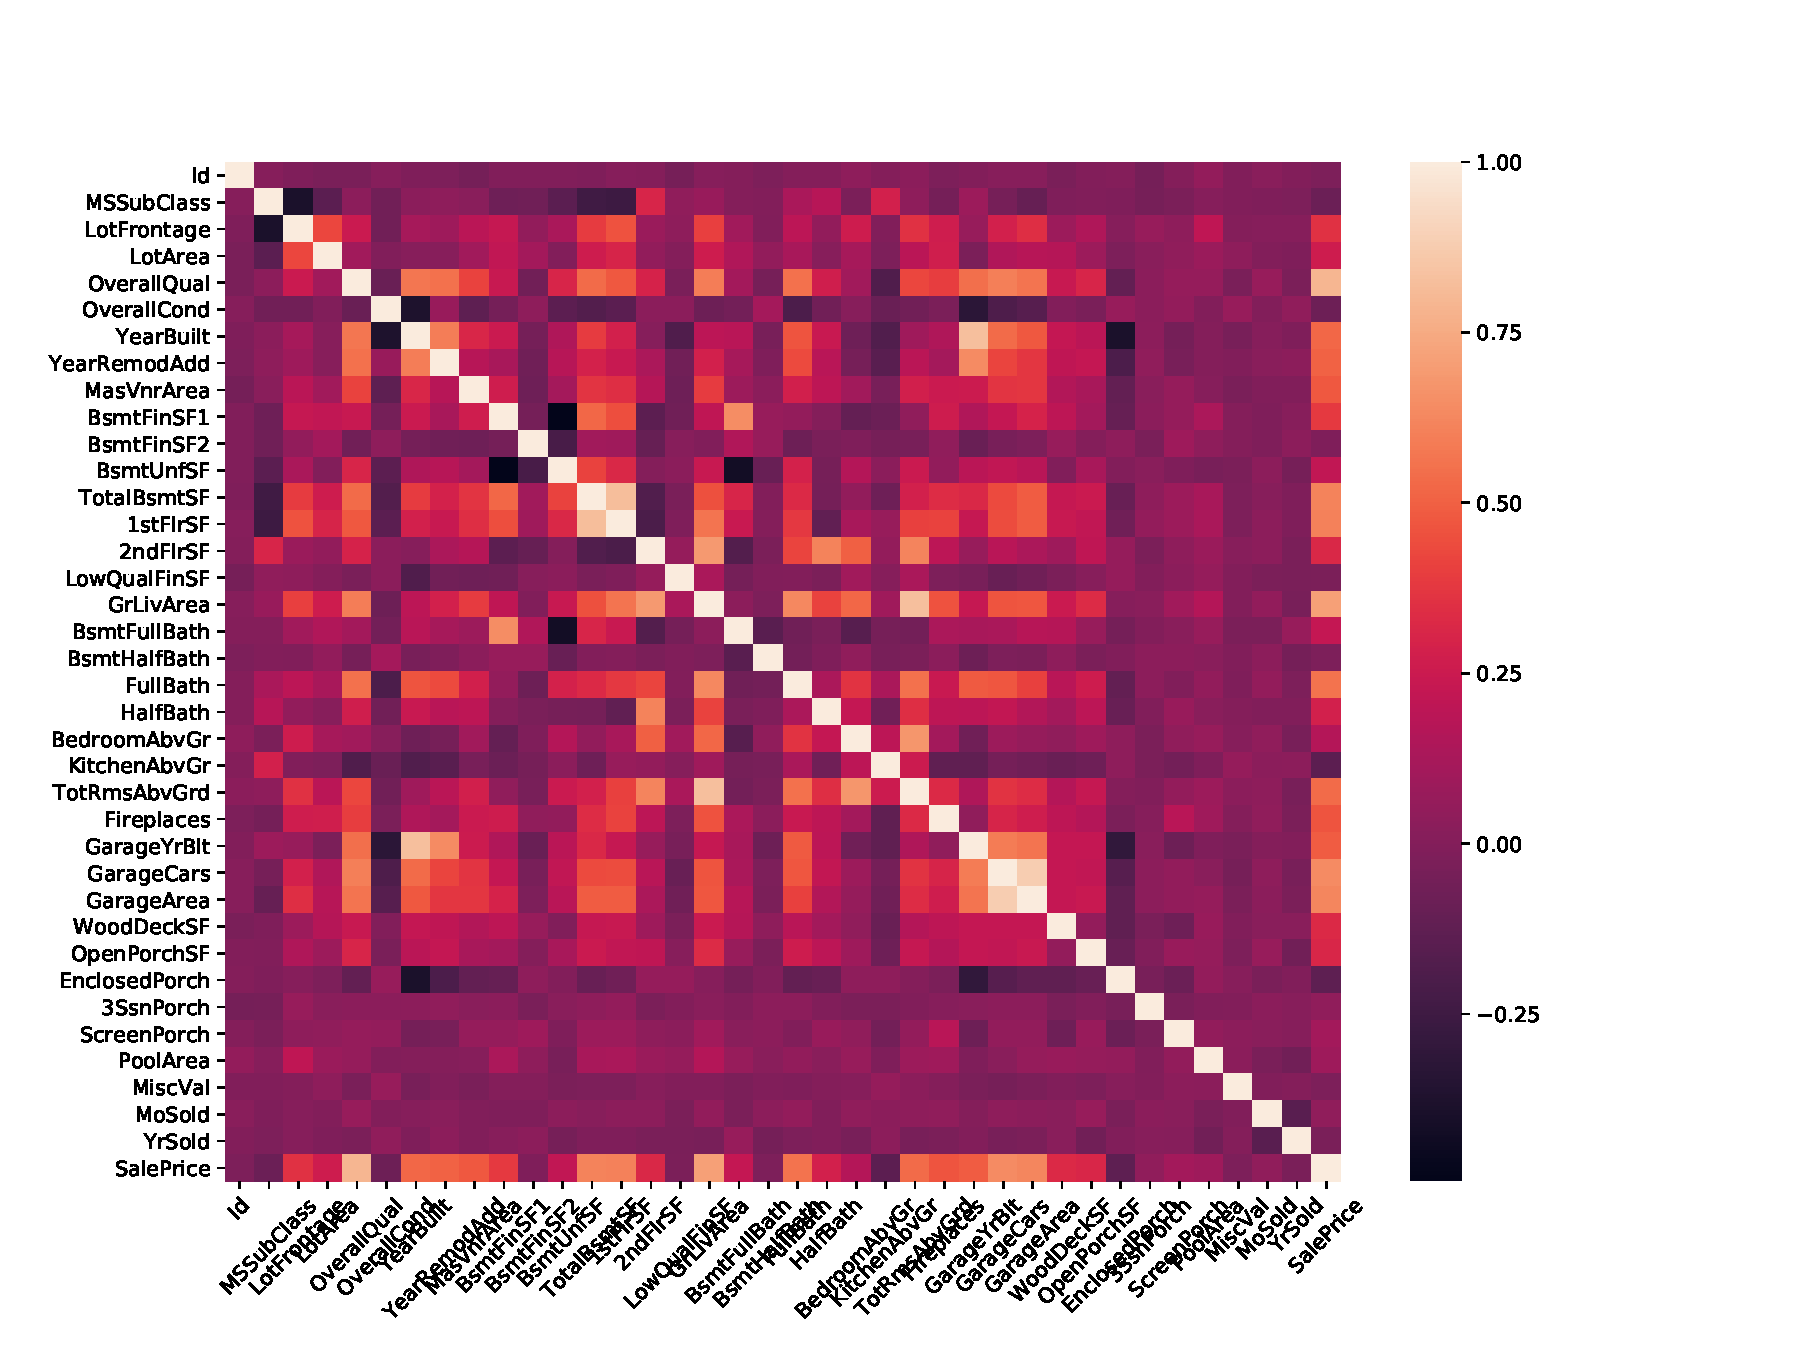
\includegraphics[scale=0.5]{imag/correlation.pdf}
		\caption{Correlación variables numéricas.}
		\label{fig:correlation_heatmap}
	\end{figure}

	Como se puede ver, las variables que más correlación tienen con SalePrice son: OverQual, GrLivArea, GarageCars, GarageArea, TotalBsmtSF, 1stFlrSF, FullBath,TotRmsAbvGrd,YearBuilt.
	
	\vspace{0.06in}
	
	Para calcular las variables categóricas más relacionadas con SalePrice, se ha utilizado el test ANOVA, después, calcularemos la disparidad de las variables haciendo log(1/resAnova[variable]). El código utilizado y las variables más relacionadas son las siguientes.
	
	\begin{lstlisting}
	def anova(frame):
	anv = pd.DataFrame()
	anv['feature'] = qualitative
	pvals = []
	for c in qualitative:
	samples = []
	for cls in frame[c].unique():
	s = frame[frame[c] == cls]['SalePrice'].values
	samples.append(s)
	pval = stats.f_oneway(*samples)[1]
	pvals.append(pval)
	anv['pval'] = pvals
	return anv.sort_values('pval')
	
	a = anova(train)
	a['disparity'] = np.log(1./a['pval'].values)
	sns.barplot(data=a, x='feature', y='disparity')
	plt.savefig('anova.pdf')
	x=plt.xticks(rotation=90)
	
	\end{lstlisting}
	
	\begin{figure}[H]
		\centering
		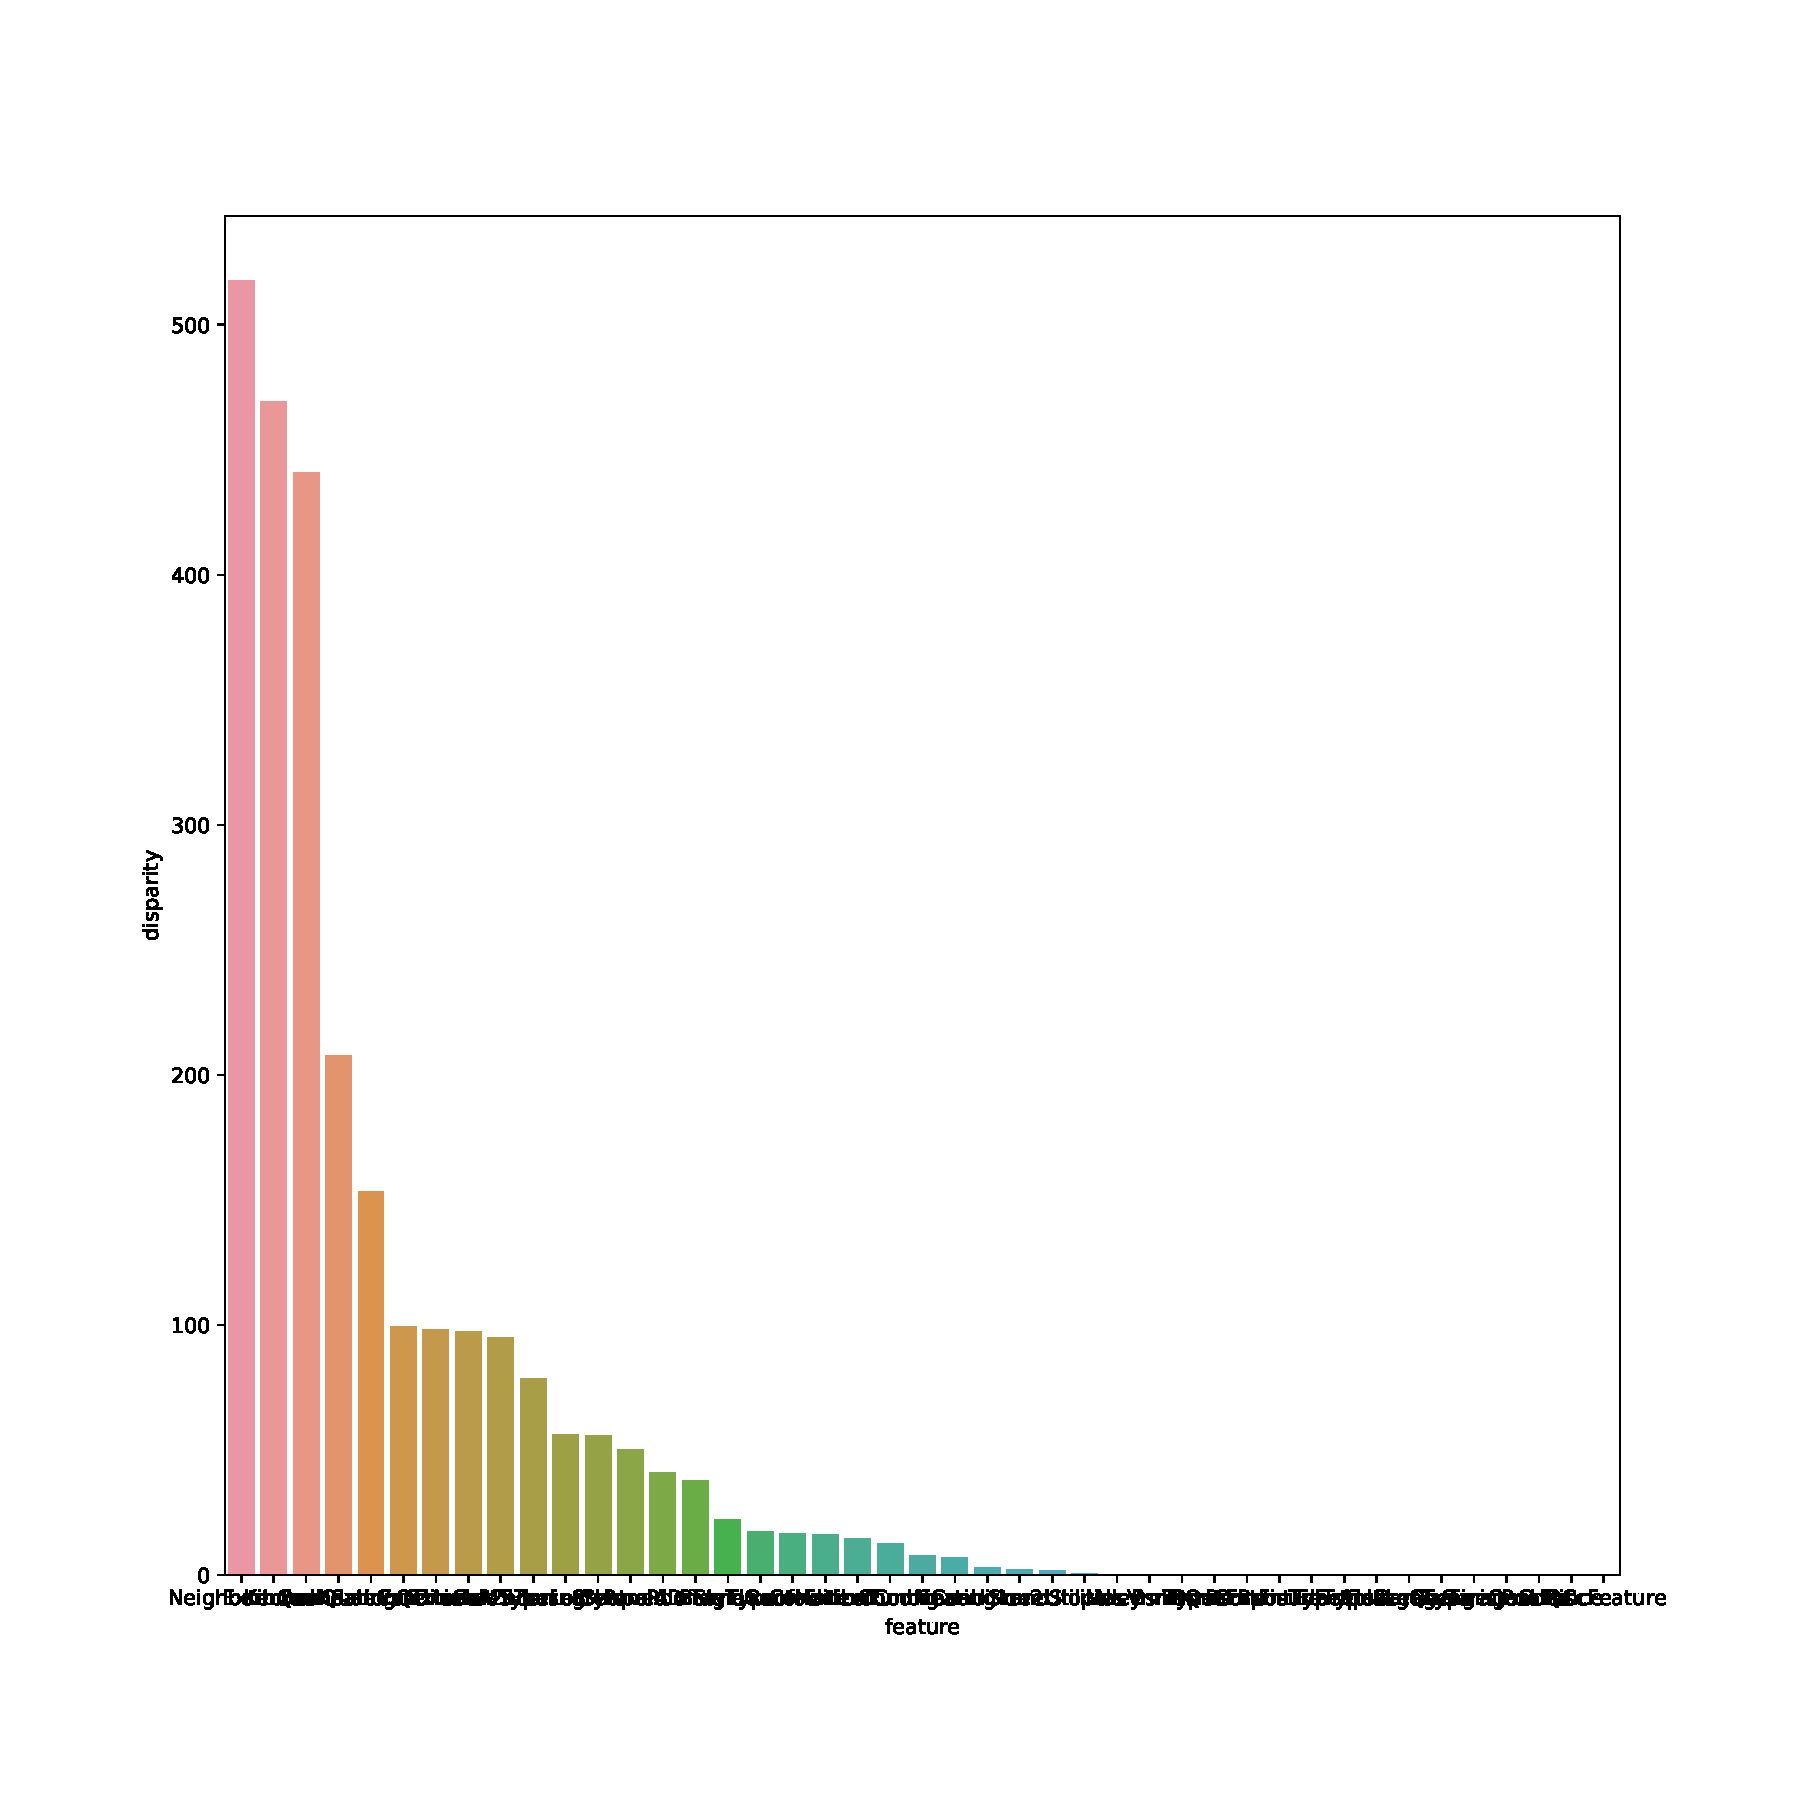
\includegraphics[scale=0.5]{imag/anova.pdf}
		\caption{Relación variables categóricas.}
		\label{fig:disparity_qualitive_data}
	\end{figure}

	Aunque en la gráfica no se pueda ver por problemas con los nombres de las variables, las variables cualitativas más importantes son: Neighborhood, ExterQual, KitchenQual, Foundation, HeatingQC, SaleCondition, Exterior1st,...
	
	\vspace{0.06in}
	Ahora que ya hemos estudiado los datos del conjunto de train, preprocesaremos los datos.
	
	\subsection{Preprocesado de datos.}
	Lo primero que haremos en este apartado será eliminar los outliers del conjunto de train, la única variable que contiene outliers es GrLivArea.
	
	\begin{figure}[H]
		\centering
		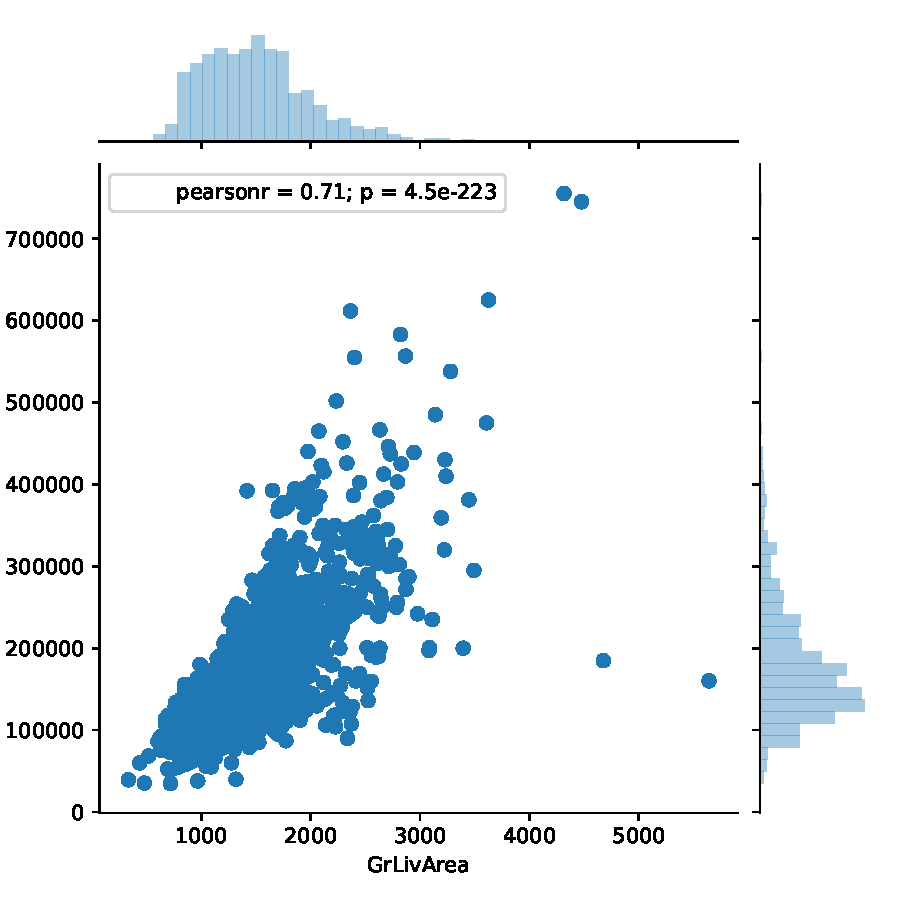
\includegraphics[scale=0.7]{imag/GrLivArea.pdf}
		\caption{Valores GrLivArea conforme a SalePrice}
		\label{fig:outliers_grlivarea}
	\end{figure}

	\vspace{0.06in}
	Como se puede ver, hay dos valores para los cuales el valor de venta de la casa es bajo para un terreno muy grande. Por ello eliminaremos esos valores.
	
	\vspace{0.06in}
	
	Lo siguiente que haremos es imputar valores pérdidos tanto para train como para test. Para ello, lo primero que haremos es unir ambos conjunto en un solo DataFrame, y después comenzaremos a imputar los valores perdidos.
	
	\vspace{0.06in}
	
	Los variables con valores perdidos son las siguientes: 'PoolQC',	'MiscFeature',
	'Alley',
	'Fence',
	'FireplaceQu',
	'LotFrontage',
	'GarageCond',
	'GarageQual',
	'GarageYrBlt',
	'GarageFinish',
	'GarageType',
	'BsmtCond',
	'BsmtExposure',
	'BsmtQual',
	'BsmtFinType2',
	'BsmtFinType1',
	'MasVnrType',
	'MasVnrArea',
	'MSZoning',
	'BsmtHalfBath',
	'Utilities',
	'Functional',
	'BsmtFullBath',
	'BsmtFinSF1',
	'Exterior1st',
	'Exterior2nd',
	'BsmtFinSF2',
	'BsmtUnfSF',
	'TotalBsmtSF',
	'SaleType',
	'Electrical',
	'KitchenQual',
	'GarageArea',
	'GarageCars'.
	
	\vspace{0.06in}
	Las variables 'Fence', 'Alley' y 'MiscFeatures' tienen muchos valores perdidos, por lo que he decidido eliminarlas.
	
	\vspace{0.06in}
	Para todas las variables numéricas, he imputado todos los valores perdidos con 0s.	
	
	\vspace{0.06in}
	Para las variables cualitativas se han empleados diferentes formas de imputar los datos. Para las variables de tipo calidad, como por ejemplo 'GarageQual', se ha creado un diccionario en python donde se representa cada uno de los diferentes valores con un número del 1 a 5, y los valores perdidos se representan con un 0.
	
	\vspace{0.06in}
	
	\begin{lstlisting}
	diccionario = {np.nan:0, "Po":1, "Fa":2, "TA":3, "Gd":4, "Ex":5}
	name = [name for name in missing_data if "QC" in name
	or "Qual" in name or "Cond" in name
	or "Qu" in name]
	
	for n in name:
		features[n] = features[n].map(diccionario).astype(int)
	\end{lstlisting}
	
	\vspace{0.06in}
	Este mismo proceso se ha seguido para las variables 'GarageFinish' y  'Utilities'. \\
	Para las variables 'BsmtFinTypeX' y 'BmstExposure' se ha optado por reemplazar los valores perdidos por los valores más votados.
	
	\vspace{0.06in}
	
	\begin{lstlisting}
	name = ["BsmtFinType2","BsmtFinType1","BsmtExposure"]
	for n in name:
		features[n] = features[n].fillna(features[n].mode()[0])
	\end{lstlisting}
	
	\vspace{0.06in}
	El mismo proceso se ha seguido para las variables 'Electrical' y  'Functional'.
	
	\vspace{0.06in}
	
	Para el resto de características que tenemos que imputar los datos, se han sustituido por valores de dentro de sus características, para ello se ha utilizado la siguiente función.
	
	\begin{lstlisting}
	from sklearn.preprocessing import LabelEncoder
	le = LabelEncoder()
	def factorize(data, var, fill_na = None):
	if fill_na is not None:
	data[var].fillna(fill_na, inplace=True)
	le.fit(data[var])
	data[var] = le.transform(data[var])
	return data
	\end{lstlisting}
	
	\vspace{0.06in}
	Lo siguiente que se hará será binarizar todas las variables cualitativas. Para ello se ha utilizado lo siguiente.
	
	\vspace{0.06in}
	
	\begin{lstlisting}
	for col in features.dtypes[features.dtypes == 'object'].index:
	for_dummy = features.pop(col)
	features = pd.concat([features, pd.get_dummies(for_dummy, prefix=col)], axis=1)
	\end{lstlisting}
	
	\vspace{0.06in}
	Lo último que haremos será modificar las variables que tienen una asimetría alta, para ello calcularemos la asimetría de cada de las variables y aquellas que tengan un valor mayor a 0.75 se modificará su valor con el logaritmo. Para usar el logaritmo se ha optado por la función log1p() ya que algunos valores tienen valores iguales a 0 y por lo tanto nos pueden ocasionar problemas a la hora de utilizarlos en los modelos. Tras esto se han estandarizado los datos con el paquete StandardScaler de sklearn.
	
	\vspace{0.06in}
	\begin{lstlisting}
		# Transformamos las variables con mucha varianza con el logaritmo.
		from scipy.stats import skew
		skewed = x_train[numeric_features].apply(lambda x: skew(x.dropna().astype(float)))
		skewed = skewed[skewed > 0.75]
		skewed = skewed.index
		
		x_train[skewed] = np.log1p(x_train[skewed])
		x_test[skewed] = np.log1p(x_test[skewed])
	\end{lstlisting}
	
	\begin{lstlisting}
		from sklearn.preprocessing import StandardScaler
		
		scaler = StandardScaler()
		scaler.fit(x_train[numeric_features])
		
		scaled = scaler.transform(x_train[numeric_features])
		for i, col in enumerate(numeric_features):
		x_train[col] = scaled[:, i]
		
		scaled = scaler.transform(x_test[numeric_features])
		for i, col in enumerate(numeric_features):
		x_test[col] = scaled[:, i]
	\end{lstlisting}
	
	\section[Resultados]{Tabla resultados en la competición.}
	\begin{tabular}{ccccccc}
		\toprule
		{} &               Nombre &        Día &          Hora & Posición & Score Kaggle & RMSLE training \\
		\midrule
		0  &       submission\_one &   27/12/17 &      19:00:00 &    \textasciitilde1000 &      0.12539 &       0.092997 \\
		1  &         submission\_x &  27- 28/12 &  varias horas &    \textasciitilde1000 &    0.13-0.15 &    0.1 – 0.078 \\
		2  &   submission\_29\_12\_2 &   29/12/17 &      13:40:00 &    \textasciitilde1000 &      0.12566 &       0.092997 \\
		3  &   Submission\_29\_12 4 &   29/12/17 &      18:20:00 &    \textasciitilde1000 &      0.12576 &       0.078509 \\
		4  &   Submission\_30 12 1 &   30/12/17 &      11:30:00 &    \textasciitilde1000 &      0.13142 &       0.050387 \\
		5  &   Submission\_30 12 2 &   30/12/17 &      14:58:00 &     \textasciitilde650 &      0.12095 &       0.075196 \\
		6  &   Submission\_30 12 3 &   30/12/17 &      14:59:00 &     \textasciitilde600 &      0.12070 &       0.073795 \\
		7  &   Submission\_30\_12 4 &   30/12/17 &      14:59:00 &     \textasciitilde580 &      0.11963 &       0.086440 \\
		8  &  Submisision\_30\_12 5 &   30/12/17 &      15:00:00 &     \textasciitilde580 &      0.12039 &       0.075087 \\
		9  &   Submission\_30\_12 6 &   30/12/17 &      15:00:00 &     \textasciitilde580 &      0.12149 &       0.073679 \\
		10 &   Submission\_30\_12 7 &   30/12/17 &      15:00:00 &     \textasciitilde580 &      0.12127 &       0.086382 \\
		11 &   Submission\_30\_12 8 &   30/12/17 &      15:02:00 &     \textasciitilde580 &      0.12127 &       0.088779 \\
		12 &   Submission\_31\_12 1 &   31/12/17 &      14:05:00 &      550 &      0.11948 &       0.083367 \\
		13 &   Submission\_31\_12 2 &   31/12/17 &      14:09:00 &      550 &      0.11992 &       0.082508 \\
		14 &   Submission\_31\_12 3 &   31/12/17 &      14:15:00 &      550 &      0.11977 &       0.085418 \\
		15 &   Submission\_31\_12 4 &   31/12/17 &      11:23:00 &      550 &      0.12028 &       0.080700 \\
		16 &   Submission\_31\_12 5 &   31/12/17 &      15:28:00 &      550 &      0.11983 &       0.080339 \\
		17 &   Submission\_31\_12 6 &   31/12/17 &      15:38:00 &      550 &      0.11994 &       0.078922 \\
		\bottomrule
	\end{tabular}

	\vspace{0.06in}

	El resto de elementos de la tabla ocupan demasiado espacio para representarlas en filas, por lo tanto, se hará un apartado por cada una de las soluciones subidas a Kaggle describiendo brevemente cada uno de los elementos.
	
	\vspace{0.06in}
	
	\subsection{Submission\_one}
	\subsubsection{Breve descripción del preprocesado.}
	El preprocesado es el que viene por defecto en el archivo ``kaggle.py``.
	\subsubsection{Breve descripción de los algoritmos utilizados.}
	Los algoritmos que se utilizan para obtener la solución son GradientBoosting y ElasticNet; para obtener la solución final, se hace una combinación de los dos, utilizando para calcular para cada uno de los precios la suma de la mita de cada una de los precios calculados.
	\subsubsection{Configuración de los parámetros de los algoritmos.}
	La configuración de los parámetros es la que viene por defecto en el archivo ``kaggle.py``
	
	\subsection{Submission\_x}
	\subsubsection{Breve descripción del preprocesado.}
	El preprocesado es el que viene por defecto en el archivo ``kaggle.py``
	\subsubsection{Breve descripción de los algoritmos utilizados.}
	Los algoritmos utilizados durante las entregas realizadas en los días 27/12 y 28/12 fueron ElasticNet, GradientBoosting, XGBoost, LightGBM. Se realizaron entregas probando la solución aportada por los algoritmos solamente o haciendo modelos complejos entre ellos.
	\subsubsection{Configuración de los parámetros de los algoritmos.}
	La configuración para ElasticNet y GradientBoosting es la misma que se aportaba en el archivo ``kaggle.py``, los algoritmos de XGBoost y LightGBM utilizan un número de estimadores igual a 3000.
	
	\subsection{Submission-29-12-2}
	\subsubsection{Breve descripción del preprocesado.}
	El preprocesado es el que viene por defecto en el archivo ``kaggle.py``.
	\subsubsection{Breve descripción de los algoritmos utilizados.}
	Los algoritmos que se utilizan para obtener la solución son GradientBoosting y ElasticNet; para obtener la solución final, se hace una combinación de los dos, utilizando para calcular para cada uno de los precios la suma de la mita de cada una de los precios calculados.
	\subsubsection{Configuración de los parámetros de los algoritmos.}
	La configuración de los parámetros es la que viene por defecto en el archivo ``kaggle.py``
	
	\subsection{Submission-29-12-4}
	\subsubsection{Breve descripción del preprocesado.}
	El preprocesado es el que viene por defecto en el archivo ``kaggle.py``.
	\subsubsection{Breve descripción de los algoritmos utilizados.}
	Para obtener la solución final, se han utilizado dos algoritmos, XGBoost y LassoCV. Para obtener la solución final, se calcula el precio de una vivienda como la suma de la mitad de cada uno de los precios calculados por los algoritmos anteriores.
	\subsubsection{Configuración de los parámetros de los algoritmos.}
	Para la configuración del algoritmo XGBoost, se han probado diferentes configuraciones, aumentando el número de estimadores, estableciendo valores diferentes para los atributos \textit{reg\_lambda} y \textit{reg\_alpha}, entre otros. Para el algoritmo de LassoCV se ha probado con cuatro valores de lambda diferentes (1, 0.1, 0.001, 0.0005).
	
	\subsection{Submission-30-12-1}
	\subsubsection{Breve descripción del preprocesado.}
	El preprocesado es el que viene por defecto en el archivo ``kaggle.py``.
	\subsubsection{Breve descripción de los algoritmos utilizados.}
	Para obtener las soluciones, se ha utiliza el algoritmo XGBoost.
	\subsubsection{Configuración de los parámetros de los algoritmos.}
	Para la configuración del algoritmo XGBoost, se han probado diferentes configuraciones, aumentando el número de estimadores, estableciendo valores diferentes para los atributos \textit{reg\_lambda} y \textit{reg\_alpha}, entre otros.
	
	\subsection{Submission-30-12-2}
	\subsubsection{Breve descripción del preprocesado.}
	Para esta solución se ha hecho una imputación de todos las variables excepto de \textit{MiscFeatures}, \textit{Alley} y \textit{Fence} que se han eliminado. También se han transformado todas las variables categóricas en numéricas, y además se han transformado aquellas variables con dispersión alta haciendo el logaritmo de estos. También se han estandarizado algunas variables de la misma forma que en el archivo ``kaggle.py``.
	\subsubsection{Breve descripción de los algoritmos utilizados.}
	Para obtener la solución final, se han utilizado dos algoritmos, XGBoost y LassoCV. Para obtener la solución final, se calcula el precio de una vivienda como la suma de la mitad de cada uno de los precios calculados por los algoritmos anteriores.
	\subsubsection{Configuración de los parámetros de los algoritmos.}
	Los parámetros utilizados son los mismos que para soluciones anteriores.
	
	\subsection{Submission-30-12-3}
	\subsubsection{Breve descripción del preprocesado.}
	Para esta solución se ha hecho una imputación de todos las variables excepto de \textit{MiscFeatures}, \textit{Alley} y \textit{Fence} que se han eliminado. También se han transformado todas las variables categóricas en numéricas, y además se han transformado aquellas variables con dispersión alta haciendo el logaritmo de estos. También se han estandarizado algunas variables de la misma forma que en el archivo ``kaggle.py``.
	\subsubsection{Breve descripción de los algoritmos utilizados.}
	Para obtener la solución final, se han utilizado los algoritmos XGBoost y LassoCV. El precio de una vivienda se calcula como la suma de la solución de XGBoost y el 90\% de la solución de LassoCV divida entre 2.
	\subsubsection{Configuración de los parámetros de los algoritmos.}
	Los parámetros utilizados son los mismos que para soluciones anteriores.
	
	\subsection{Submission-30-12-4}
	\subsubsection{Breve descripción del preprocesado.}
	Para esta solución se ha hecho una imputación de todos las variables excepto de \textit{MiscFeatures}, \textit{Alley} y \textit{Fence} que se han eliminado. También se han transformado todas las variables categóricas en numéricas, y además se han transformado aquellas variables con dispersión alta haciendo el logaritmo de estos. También se han estandarizado algunas variables de la misma forma que en el archivo ``kaggle.py``.
	\subsubsection{Breve descripción de los algoritmos utilizados.}
		Para obtener la solución final, se han utilizado los algoritmos XGBoost y LassoCV. El precio de una vivienda se calcula como la suma del 30\% del precio calculado por XGBoost y un 70\% del precio calculado por LassoCV.
	\subsubsection{Configuración de los parámetros de los algoritmos.}
	Los parámetros utilizados son los mismos que para soluciones anteriores.
	
	\subsection{Submission-30-12-5}
	\subsubsection{Breve descripción del preprocesado.}
	Para esta solución se ha hecho una imputación de todos las variables excepto de \textit{MiscFeatures}, \textit{Alley} y \textit{Fence} que se han eliminado. También se han transformado todas las variables categóricas en numéricas, y además se han transformado aquellas variables con dispersión alta haciendo el logaritmo de estos. También se han estandarizado algunas variables de la misma forma que en el archivo ``kaggle.py``.
	\subsubsection{Breve descripción de los algoritmos utilizados.}
		Para obtener la solución final, se han utilizado dos algoritmos, XGBoost y LassoCV. Para obtener la solución final, se calcula el precio de una vivienda como la suma de la mitad de cada uno de los precios calculados por los algoritmos anteriores.
	\subsubsection{Configuración de los parámetros de los algoritmos.}
	Para esta solución, se han añadido un nuevo alpha al algorimto LassoCV, el nuevo valor es 0.00099.
	
	\subsection{Submission-30-12-6}
	\subsubsection{Breve descripción del preprocesado.}
	Para esta solución se ha hecho una imputación de todos las variables excepto de \textit{MiscFeatures}, \textit{Alley} y \textit{Fence} que se han eliminado. También se han transformado todas las variables categóricas en numéricas, y además se han transformado aquellas variables con dispersión alta haciendo el logaritmo de estos. También se han estandarizado algunas variables de la misma forma que en el archivo ``kaggle.py``.
	\subsubsection{Breve descripción de los algoritmos utilizados.}
		Para obtener la solución final, se han utilizado los algoritmos XGBoost y LassoCV. El precio de una vivienda se calcula como la suma de la solución de XGBoost y el 90\% de la solución de LassoCV divida entre 2.
	\subsubsection{Configuración de los parámetros de los algoritmos.}
	La configuración es igual que para la solución \textbf{Submission-30-12-5}.
	
	\subsection{Submission-30-12-7}
	\subsubsection{Breve descripción del preprocesado.}
	Para esta solución se ha hecho una imputación de todos las variables excepto de \textit{MiscFeatures}, \textit{Alley} y \textit{Fence} que se han eliminado. También se han transformado todas las variables categóricas en numéricas, y además se han transformado aquellas variables con dispersión alta haciendo el logaritmo de estos. También se han estandarizado algunas variables de la misma forma que en el archivo ``kaggle.py``.
	\subsubsection{Breve descripción de los algoritmos utilizados.}
		Para obtener la solución final, se han utilizado los algoritmos XGBoost y LassoCV. El precio de una vivienda se calcula como la suma del 30\% del precio calculado por XGBoost y un 70\% del precio calculado por LassoCV.
	\subsubsection{Configuración de los parámetros de los algoritmos.}
		La configuración es igual que para la solución \textbf{Submission-30-12-5}.
	
	
	\subsection{Submission-30-12-8}
	\subsubsection{Breve descripción del preprocesado.}
	Para esta solución se ha hecho una imputación de todos las variables excepto de \textit{MiscFeatures}, \textit{Alley} y \textit{Fence} que se han eliminado. También se han transformado todas las variables categóricas en numéricas, y además se han transformado aquellas variables con dispersión alta haciendo el logaritmo de estos. También se han estandarizado algunas variables de la misma forma que en el archivo ``kaggle.py``.
	\subsubsection{Breve descripción de los algoritmos utilizados.}
	Para obtener la solución final, se han utilizado los algoritmos XGBoost y Lasso El precio de una vivienda se calcula como la suma del 30\% del precio calculado por XGBoost y un 70\% del precio calculado por Lasso
	\subsubsection{Configuración de los parámetros de los algoritmos.}
	Para el algoritmo Lasso, se ha utilizado un valor de lambda = 0.00099 y el número máximo de iteraciones es 50000.
	
	
	\subsection{Submission-31-12-1}
	\subsubsection{Breve descripción del preprocesado.}
	Se ha utiliza el paquete StandardScaler para estandarizar los datos en vez del estandarizado que se utilizaba en el archivo ``kaggle.py``. Además ahora todos los algoritmos utilizan los datos estandarizados. La transformación logarítmica de las variables con asimetría alta se hace con la función log1p para evitar problemas con 0 para algunos datos.
	\subsubsection{Breve descripción de los algoritmos utilizados.}
	Para obtener la solución final, se han utilizado los algoritmos XGBoost y LassoCV. El precio de una vivienda se calcula como la suma del 30\% del precio calculado por XGBoost y un 70\% del precio calculado por LassoCV.
	\subsubsection{Configuración de los parámetros de los algoritmos.}
	Los parámetros utilizados para obtener la solución son los mismos que se han utilizado para \textbf{Submission-30-12-4} y anteriores.
	
	
	\subsection{Submission-31-12-2}
	\subsubsection{Breve descripción del preprocesado.}
	Es igual que para \textbf{Submission-31-12-1}.
	\subsubsection{Breve descripción de los algoritmos utilizados.}
	Para obtener la solución final, se han utilizado los algoritmos XGBoost y LassoCV. El precio de una vivienda se calcula como la suma de la solución de XGBoost y el 90\% de la solución de LassoCV divida entre 2.
	\subsubsection{Configuración de los parámetros de los algoritmos.}
	Los parámetros utilizados para obtener la solución son los mismos que se han utilizado para \textbf{Submission-30-12-4} y anteriores.
	
	
	\subsection{Submission-31-12-3}
	\subsubsection{Breve descripción del preprocesado.}
	Es igual que para \textbf{Submission-31-12-1}.
	\subsubsection{Breve descripción de los algoritmos utilizados.}
		Para obtener la solución final, se han utilizado dos algoritmos, XGBoost y LassoCV. Para obtener la solución final, se calcula el precio de una vivienda como la suma de la mitad de cada uno de los precios calculados por los algoritmos anteriores.
	\subsubsection{Configuración de los parámetros de los algoritmos.}
	Los parámetros utilizados para obtener la solución son los mismos que se han utilizado para \textbf{Submission-30-12-4} y anteriores.
	
	\subsection{Submission-31-12-4}
	\subsubsection{Breve descripción del preprocesado.}
	Es igual que para \textbf{Submission-31-12-1}.
	\subsubsection{Breve descripción de los algoritmos utilizados.}
	Para obtener las soluciones se utilizan los algoritmos LassoCV, XGBoost y ElasticNet. Para obtener el valor de una vivienda se suma el 30\% del precio calculado por XGBoost, un 40\% del precio calculado por LassoCV y el resto por el precio calculado por ElasticNet.
	\subsubsection{Configuración de los parámetros de los algoritmos.}
	Los parámetros utilizados para obtener la solución son los mismos que se han utilizado para \textbf{Submission-30-12-4} y anteriores. Para el algoritmo de ElasticNet se han utilizado los mismos parámetros que se utilizan en ``kaggle.py``
	
	\subsection{Submission-31-12-5}
	\subsubsection{Breve descripción del preprocesado.}
	Es igual que para \textbf{Submission-31-12-1}.
	\subsubsection{Breve descripción de los algoritmos utilizados.}
	Para obtener las soluciones se utilizan los algoritmos LassoCV, XGBoost y ElasticNet. Para obtener el valor de una vivienda se suma el 30\% del precio calculado por XGBoost, un 45\% del precio calculado por LassoCV y el resto por el precio calculado por ElasticNet.
	\subsubsection{Configuración de los parámetros de los algoritmos.}
	Los parámetros utilizados para obtener la solución son los mismos que se han utilizado para \textbf{Submission-30-12-4} y anteriores. Para el algoritmo de ElasticNet se han utilizado los mismos parámetros que se utilizan en ``kaggle.py``
	
	\subsection{Submission-31-12-6}
	\subsubsection{Breve descripción del preprocesado.}
	Es igual que para \textbf{Submission-31-12-1}.
	\subsubsection{Breve descripción de los algoritmos utilizados.}
	Para obtener las soluciones se utilizan los algoritmos LassoCV, XGBoost y ElasticNet. Para obtener el precio de una vivienda, se calcula la suma de los precios obtenidos por los algoritmos y se divide entre 3.
	\subsubsection{Configuración de los parámetros de los algoritmos.}
	Los parámetros utilizados para obtener la solución son los mismos que se han utilizado para \textbf{Submission-30-12-4} y anteriores. Para el algoritmo de ElasticNet se han utilizado los mismos parámetros que se utilizan en ``kaggle.py``
	
	\section{Distribución de las soluciones entregadas.}
	Por cada una de las soluciones que se han comentado antes, se ha proporciona una carpeta que contiene el archivo submissionxxx.csv y el script de python que se ha utilizado para obtener la solución.
	
	\vspace{0.06in}
	Para algunos casos para los cuáles dentro del script de python solamente cambia cómo se calcula la solución final, se ha guardado en un mismo directorio los 3 archivos .csv que se pueden obtener y el script de python. Dentro del script se puede descomentar y comentar las líneas que calculan las solución para obtener las diferentes soluciones si se desea.

\end{document}